\newcommand{\wormTagResultsAucTable}{
    \begin{table}[H]
        \centering
        \begin{tabular}{|p{2,8cm}||p{2,8cm} p{2,8cm} p{2,8cm}|}
            \hline
            Worm Tag & ALOHA & Joint Embedding & Proposed Model \\
            \hline
            AUC-ROC & \textBF{0.962$\pm$0.003} & 0.957$\pm$0.014 & 0.946$\pm$0.018 \\
            \hline
        \end{tabular}
        \caption{AUC-ROC (Area Under Curve) of the different models for the \textbf{Worm Tag} prediction task. Results were aggregated over \textBF{3} training runs with different weight initializations and minibatch orderings. Best results are shown in \textbf{bold}.} \label{tab:wormTag_auc}
    \end{table}
}

\newcommand{\wormTagResultsAtFprTable}{
    \begin{center}
        \begin{longtable}[c]{|p{3,2cm}||p{1,8cm} p{1,8cm} p{1,8cm} p{1,8cm} p{1,8cm}|}
            \hline
            Worm Tag & \multicolumn{5}{c|}{{FPR}} \\
            & $10^{-5}$ & $10^{-4}$ & $10^{-3}$ & $10^{-2}$ & $10^{-1}$ \\
            \hline
            \endfirsthead

            \caption*{\raggedright ...continued from previous page} \\
            \hline
            Worm Tag & \multicolumn{5}{c|}{\textbf{FPR}} \\
            & $10^{-5}$ & $10^{-4}$ & $10^{-3}$ & $10^{-2}$ & $10^{-1}$ \\
            \hline
            \endhead

            \caption*{\raggedleft ...continued on next page} \\
            \endfoot

            \caption{Mean and standard deviation results (TPR, Accuracy, Recall, Precision and F1-Score) of the different models for the \textbf{Worm Tag} prediction task at different \textbf{FPR}s (\textit{False Positive Rates}). Results were aggregated over \textBF{3} training runs with different weight initializations and minibatch orderings. Best results are shown in \textbf{bold}. Under \textbf{TPR} results are also presented the percentage reduction in mean detection error and in ROC curve standard deviation introduced by the \textit{Proposed Model} with respect to both \textit{ALOHA} model and \textit{Joint Embedding}.} \label{tab:wormTag_results_at_fpr} \\
            \endlastfoot

            \multicolumn{6}{|c|}{\textbf{TPR}} \\
            \hline
            ALOHA & 0.116$\pm$0.066 & 0.197$\pm$0.123 & 0.489$\pm$0.049 & 0.652$\pm$0.014 & 0.813$\pm$0.026 \\
            Joint Embedding & \textBF{0.236$\pm$0.127} & 0.357$\pm$0.118 & 0.532$\pm$0.005 & 0.649$\pm$0.005 & \textBF{0.831$\pm$0.069} \\
            Proposed Model & 0.228$\pm$0.019 & \textBF{0.378$\pm$0.094} & \textBF{0.548$\pm$0.031} & \textBF{0.654$\pm$0.025} & 0.808$\pm$0.047 \\
            \hline
            Error Reduction wrt \newline ALOHA & 12.7\% & 22.5\% & 11.5\% & 0.6\% & -2.7\% \\
            Error Reduction wrt \newline Joint Embedding & -1.0\% & 3.3\% & 3.4\% & 1.4\% & -13.6\% \\
            \hline
            Std Reduction wrt \newline ALOHA & 71.2\% & 23.6\% & 36.7\% & -78.6\% & -80.8\% \\
            Std Reduction wrt \newline Joint Embedding & 85.0\% & 20.3\% & -520.0\% & -400.0\% & 31.9\% \\
            \hline
            \multicolumn{6}{|c|}{\textbf{Accuracy}} \\
            \hline
            ALOHA & 0.860$\pm$0.010 & 0.873$\pm$0.019 & 0.918$\pm$0.008 & 0.936$\pm$0.002 & 0.886$\pm$0.004 \\
            Joint Embedding & \textBF{0.879$\pm$0.020} & 0.898$\pm$0.019 & 0.925$\pm$0.001 & 0.936$\pm$0.001 & \textBF{0.889$\pm$0.011} \\
            Proposed Model & 0.878$\pm$0.003 & \textBF{0.901$\pm$0.015} & \textBF{0.928$\pm$0.005} & \textBF{0.937$\pm$0.004} & 0.885$\pm$0.008 \\
            \hline
            \multicolumn{6}{|c|}{\textbf{Recall}} \\
            \hline
            ALOHA & 0.116$\pm$0.066 & 0.197$\pm$0.123 & 0.489$\pm$0.049 & 0.652$\pm$0.014 & 0.813$\pm$0.026 \\
            Joint Embedding & \textBF{0.236$\pm$0.127} & 0.357$\pm$0.118 & 0.532$\pm$0.005 & 0.649$\pm$0.005 & \textBF{0.831$\pm$0.069} \\
            Proposed Model & 0.228$\pm$0.019 & \textBF{0.378$\pm$0.094} & \textBF{0.548$\pm$0.031} & \textBF{0.654$\pm$0.025} & 0.808$\pm$0.047 \\
            \hline
            \multicolumn{6}{|c|}{\textbf{Precision}} \\
            \hline
            ALOHA & 0.999$\pm$0.000 & 0.996$\pm$0.002 & 0.989$\pm$0.001 & \textBF{0.925$\pm$0.002} & 0.605$\pm$0.008 \\
            Joint Embedding & \textBF{1.000$\pm$0.000} & 0.998$\pm$0.001 & \textBF{0.990$\pm$0.000} & 0.924$\pm$0.001 & \textBF{0.609$\pm$0.020} \\
            Proposed Model & \textBF{1.000$\pm$0.000} & \textBF{0.999$\pm$0.000} & 0.990$\pm$0.001 & 0.925$\pm$0.003 & 0.603$\pm$0.014 \\
            \hline
            \multicolumn{6}{|c|}{\textbf{F1 Score}} \\
            \hline
            ALOHA & 0.202$\pm$0.102 & 0.313$\pm$0.162 & 0.653$\pm$0.045 & 0.764$\pm$0.010 & 0.694$\pm$0.014 \\
            Joint Embedding & 0.365$\pm$0.162 & 0.515$\pm$0.134 & 0.692$\pm$0.004 & 0.763$\pm$0.004 & \textBF{0.703$\pm$0.038} \\
            Proposed Model & \textBF{0.372$\pm$0.025} & \textBF{0.542$\pm$0.094} & \textBF{0.705$\pm$0.026} & \textBF{0.766$\pm$0.018} & 0.690$\pm$0.026 \\
            \hline
        \end{longtable}
    \end{center}
}

\newcommand{\wormTagResultsSummaryTable}{
    \begin{table}[H]
        \centering
        \begin{tabular}{|p{3,2cm}||p{1,8cm} p{1,8cm} p{1,8cm} p{1,8cm} p{1,8cm}|}
            \hline
            \multicolumn{6}{|c|}{Worm Tag (at FPR $=1\%$)} \\
            \hline
            Model & TPR & Accuracy & Precision & Recall & F1 score \\
            \hline
            ALOHA & 0.652$\pm$0.014 & 0.936$\pm$0.002 & \textBF{0.925$\pm$0.002} & 0.652$\pm$0.014 & 0.764$\pm$0.010 \\
            Joint Embedding & 0.649$\pm$0.005 & 0.936$\pm$0.001 & 0.924$\pm$0.001 & 0.649$\pm$0.005 & 0.763$\pm$0.004 \\
            Proposed Model & \textBF{0.654$\pm$0.025} & \textBF{0.937$\pm$0.004} & 0.925$\pm$0.003 & \textBF{0.654$\pm$0.025} & \textBF{0.766$\pm$0.018} \\
            \hline
        \end{tabular}
        \caption{Summary of the mean and standard deviation results of the different models for the \textbf{Worm Tag} prediction task at \textbf{FPR} $=1\%$. Results were aggregated over \textBF{3} training runs with different weight initializations and minibatch orderings. Best results are shown in \textbf{bold}.} \label{tab:wormTag_result_summary}
    \end{table}
}

\newcommand{\wormTagRocAloha}{
    \begin{figure}[H]
        \vspace*{-0.5cm}
        \centering
        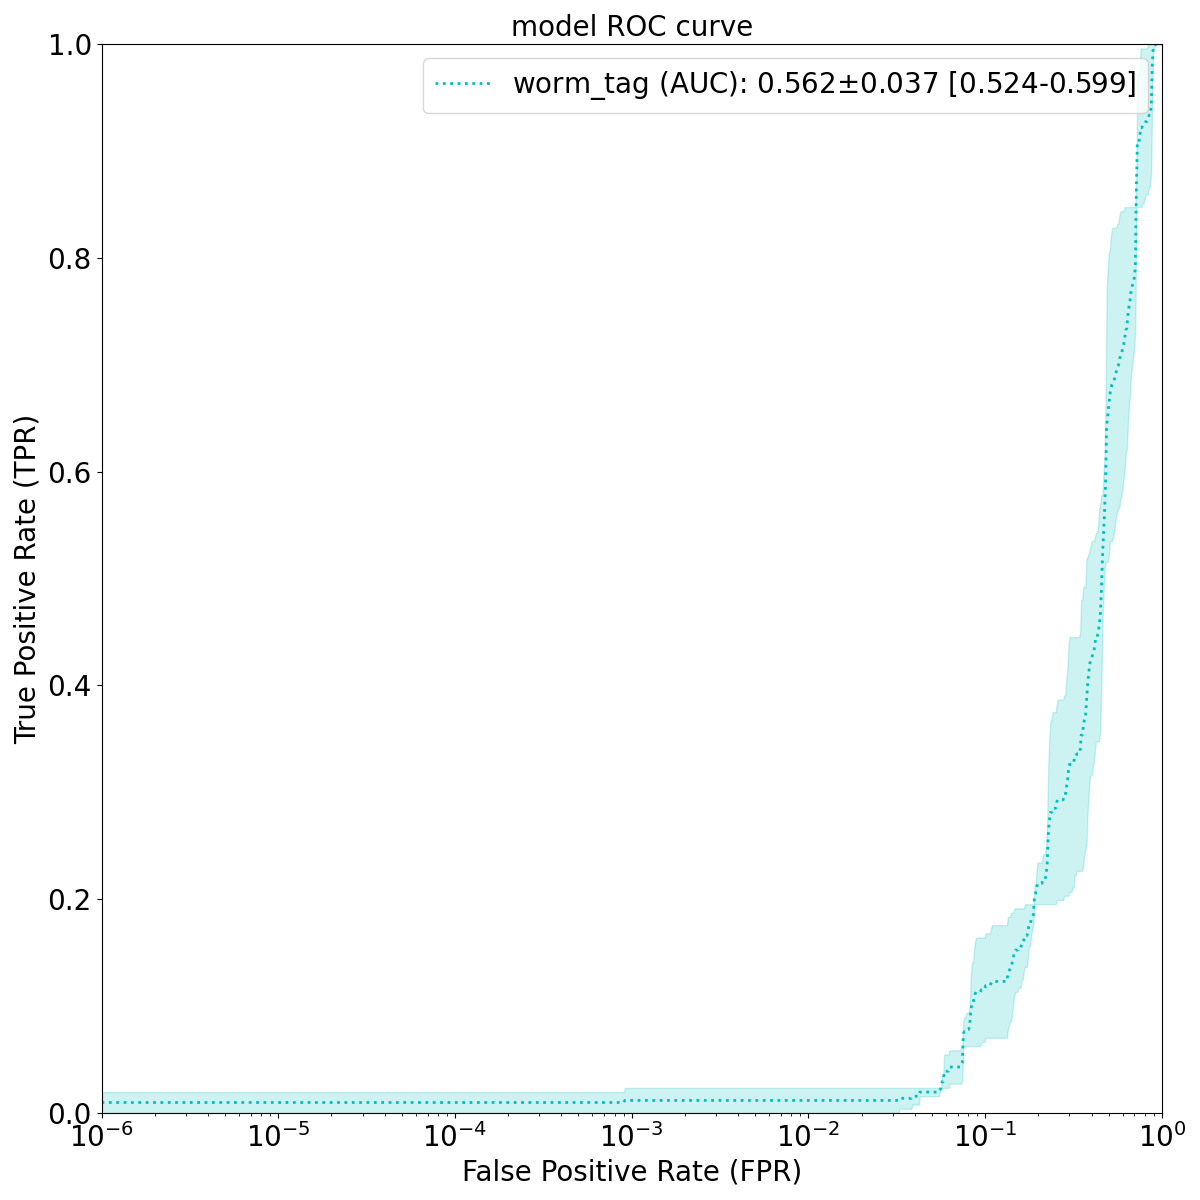
\includegraphics[width=0.6\textwidth]{./results/worm_tag_roc_aloha.png}
        \vspace*{-0.2cm}
        \caption{ROC curve and AUC statistics of \textBF{ALOHA} model for the \textbf{Worm Tag}. The line represents the \textit{mean} TPR at a given FPR, while the shaded region represents the \textit{standard deviation}. Statistics were computed over \textBF{3} training runs, each with random parameter initialization.}
        \label{fig:wormTagRocAloha}
    \end{figure}
}

\newcommand{\wormTagRocJointEmbedding}{
    \begin{figure}[H]
        \vspace*{-0.5cm}
        \centering
        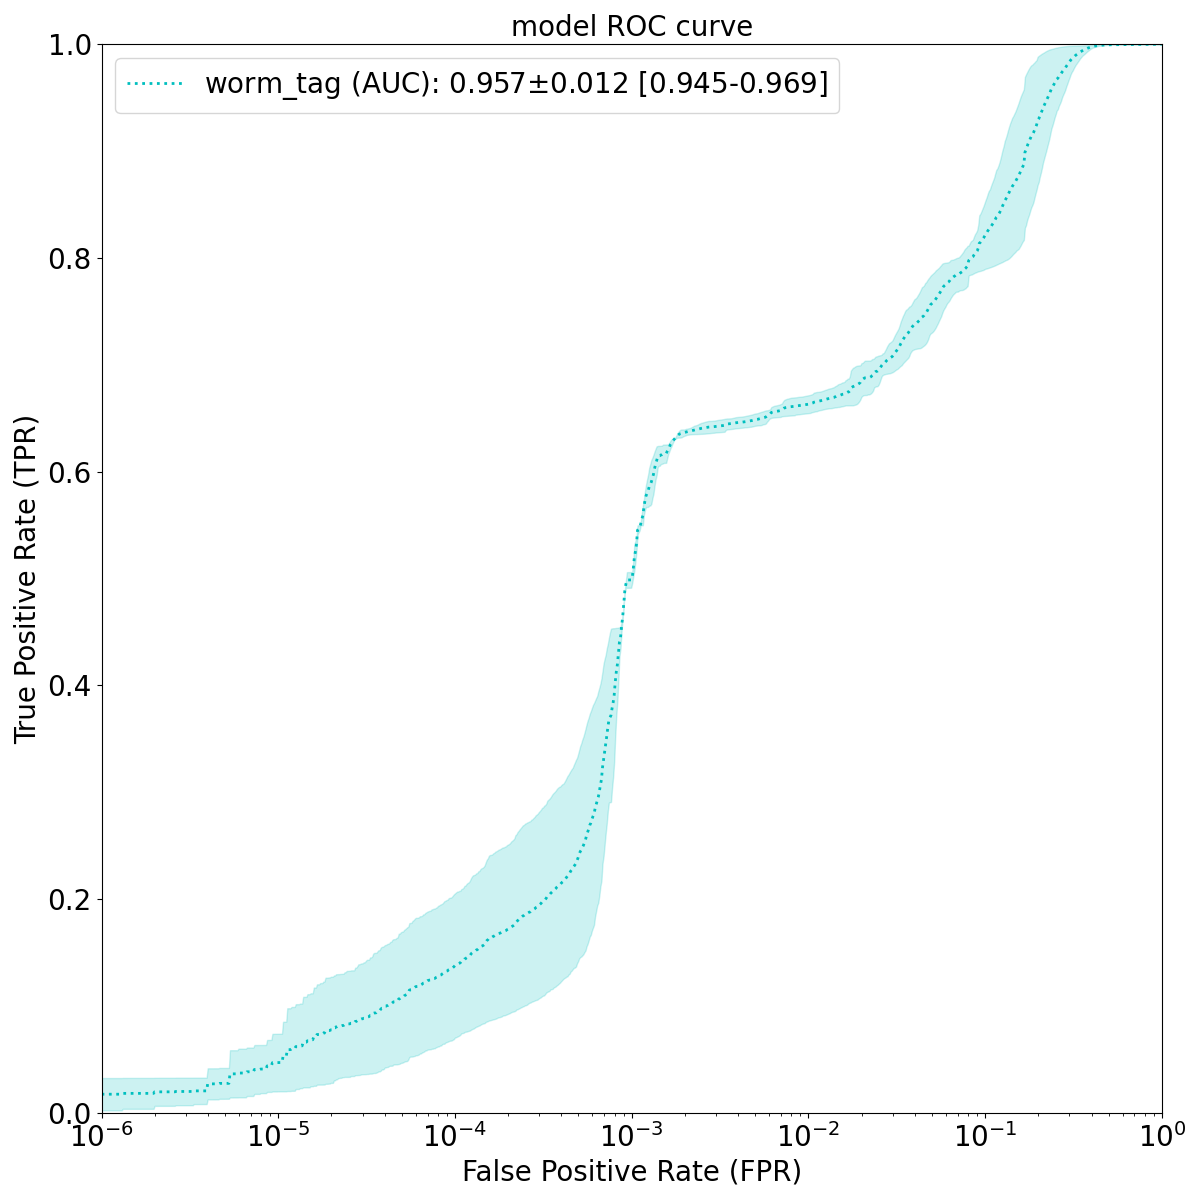
\includegraphics[width=0.6\textwidth]{./results/worm_tag_roc_jointEmbedding.png}
        \vspace*{-0.2cm}
        \caption{ROC curve and AUC statistics of \textBF{Joint Embedding} model for the \textbf{Worm Tag}. The line represents the \textit{mean} TPR at a given FPR, while the shaded region represents the \textit{standard deviation}. Statistics were computed over \textBF{3} training runs, each with random parameter initialization.}
        \label{fig:wormTagRocJointEmbedding}
    \end{figure}
}

\newcommand{\wormTagRocProposedMethod}{
    \begin{figure}[H]
        \vspace*{-0.5cm}
        \centering
        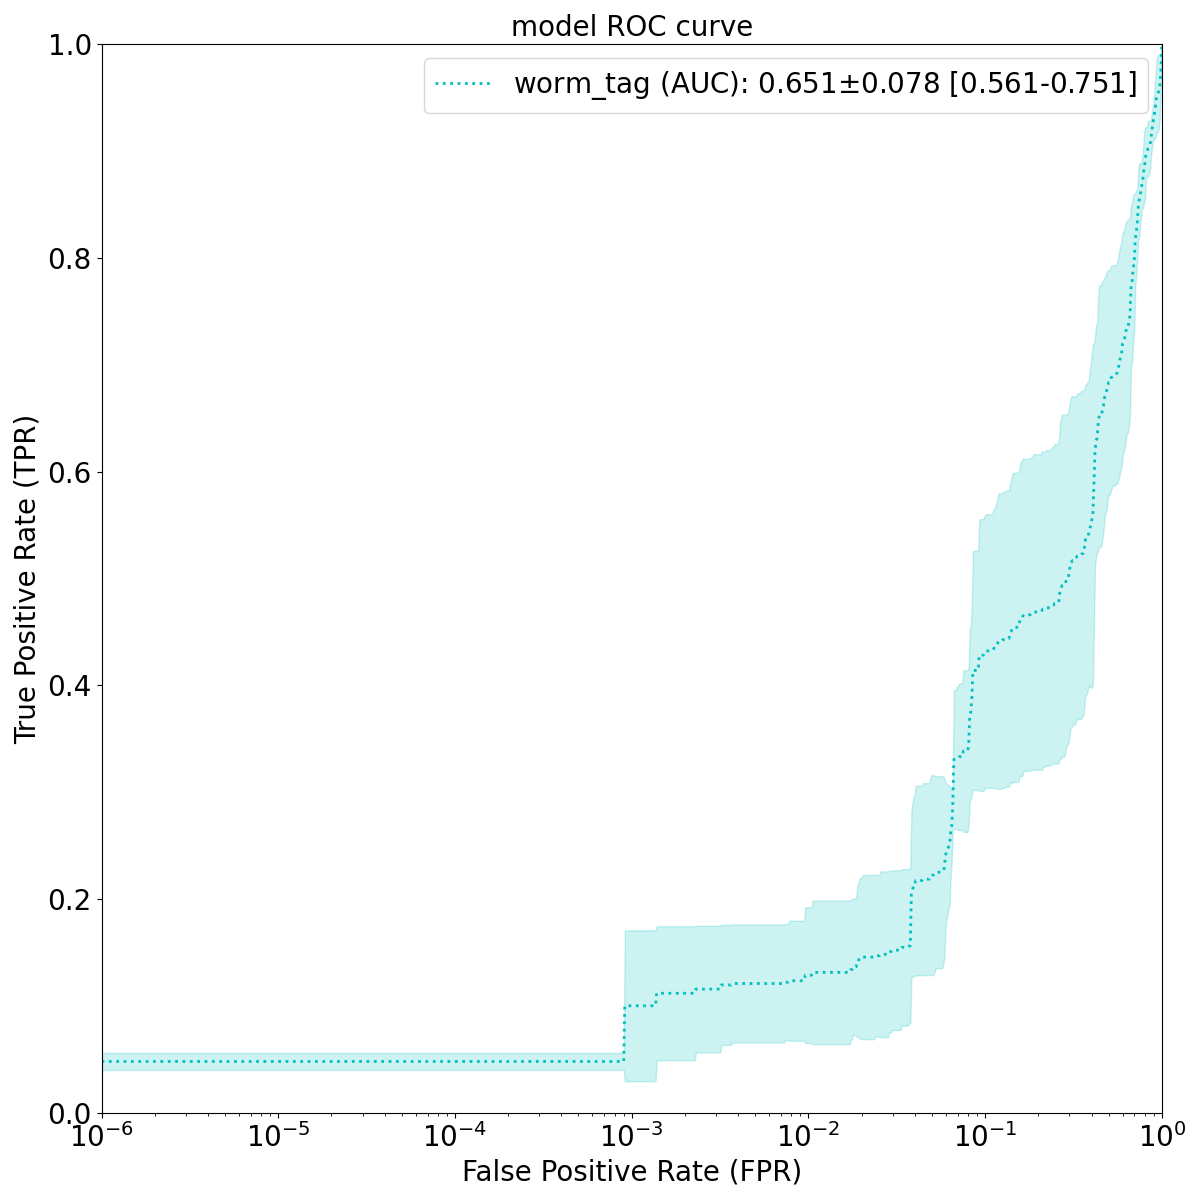
\includegraphics[width=0.6\textwidth]{./results/worm_tag_roc_proposedModel.png}
        \vspace*{-0.2cm}
        \caption{ROC curve and AUC statistics of \textBF{Proposed Model} for the \textbf{Worm Tag}. The line represents the \textit{mean} TPR at a given FPR, while the shaded region represents the \textit{standard deviation}. Statistics were computed over \textBF{3} training runs, each with random parameter initialization.}
        \label{fig:wormTagRocProposedModel}
    \end{figure}
}
